\chapter{Computer Vision}


% ---------- Computer Vision Sample Metric ----------
\clearpage
\thispagestyle{cvstyle}
\section{Computer Vision Sample Metric}
\subsection{Computer Vision Sample Metric}


% ---------- PSNR ----------
\clearpage
\thispagestyle{cvstyle}
\section{PSNR}
\subsection{Peak Signal-to-Noise Ratio}

In image generation and reconstruction, it is important to measure how closely the generated images resemble reference images.
PSNR is a widely used metric that quantifies pixel-level differences.

% equation
\begin{center}
    \tikz{
        \node[inner sep=2pt, font=\Large] (a) {
            {
                $\displaystyle
                    PSNR = 10 \cdot \log_{10}\left(\frac{\color{nmlred}MAX^2}{\color{nmlpurple}MSE}\right)
                $
            }
        };
        \draw[-latex,nmlred, semithick] ($(a.north)+(2.1,-0)$) to[bend right=15] node[pos=1, left] {maximum possible pixel} +(-1,.5); 
        \draw[-latex,nmlpurple, semithick] ($(a.south)+(2,-0.1)$) to[bend left=15] node[pos=1, left] {mean squared error} +(-1,-.5);
    }
\end{center}

\vspace{-10pt} 

where given an original image $O$ of size $h \times w$ and a reconstructed image $R$, the $MSE$ is defined as:

\vspace{-10pt}

% equation
\begin{center}
    \tikz{
        \node[inner sep=2pt, font=\large] (a) {
            {
                $\displaystyle
                 MSE = \frac{1}{\color{teal!70!green}h \cdot \color{nmlcyan}w} \sum_{i=1}^{h} \sum_{j=1}^{w} \left(\color{nmlred} O(i,j) \color{black} - \color{nmlpurple} R(i,j) \right)^2
                $
            }
        };
        \draw[-latex,teal!70!green, semithick] ($(a.west)+(1.7,-0.5)$) to[bend left=15] node[pos=1, left] {height} +(-1,-.5); 
        \draw[-latex,nmlcyan, semithick] ($(a.west)+(2.4,-0.5)$) to[bend right=15] node[pos=1.62, left] {width} +(1,-.5);
        \draw[-latex,nmlred, semithick] ($(a.south)+(1,0.5)$) to[bend right=15] node[pos=1, right] {original pixel value} +(1,-.5);
        \draw[-latex,nmlpurple, semithick] ($(a.north)+(2.3,-0.4)$) to[bend right=15] node[pos=1, left] {reconstructed pixel value} +(-1,.5);    
    }
\end{center}

\vspace{-10pt}

The intuition behind PSNR is that it expresses how large the possible signal value is in comparison to the error. 
If the error is subtle compared to the maximum signal (i.e., a high PSNR), the reconstructed image is relatively similar to the target in terms of pixel values.
The unit of peak signal-to-noise ratio is decibel (dB) and the image have PSNR from 30 dB could be consider as good reconstruction quality.



\textbf{When to use PSNR?}

PSNR is often chosen as the first metric to provide an overview of how closely the generated image matches the target.

\coloredboxes{
\item It is a straightforward and widely accepted standard for comparing vision algorithms.
\item Simple and fast to compute.
}
{
\item It is not always align with human perception of image.
\item PSNR is sensitive to even small global changes in lighting, contrast, or color.
}

\clearpage

\thispagestyle{customstyle}


\begin{figure*}[ht!]
    \centering
    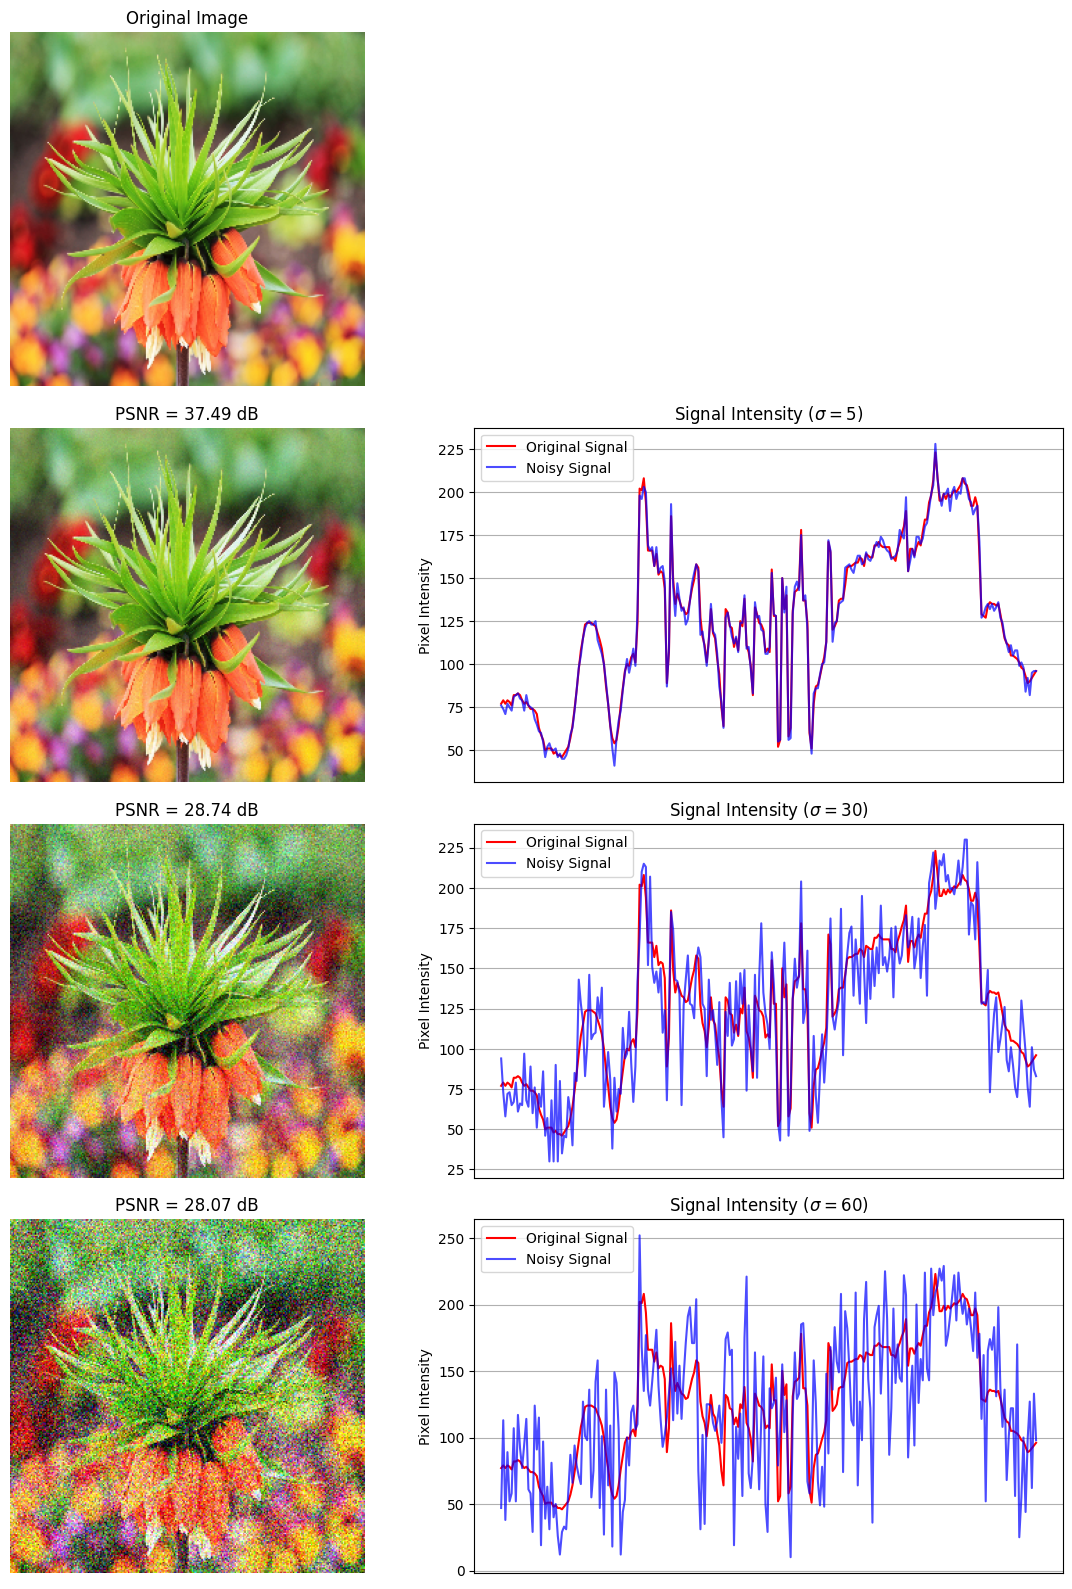
\includegraphics[width=0.6\textwidth]{figures/PSNR_plot.png}
    % \caption{Caption}
    \label{PSNR plot}
\end{figure*}


\textbf{Figure 7.1 Image with different PSNR.} Demonstrates noisy images with their corresponding PSNR values compared to the original ones. \textbf{Left:} Original image and its noisy version. 
\textbf{Right:} Illustration of how strong noise signals have been added to the original image.

\vspace{-10pt} 

\orangebox{Did you know that...}
{PSNR is not just for images; it can be applied to \textbf{video, audio, or even signal processing}. Anytime we want to measure the quality of \textbf{reconstructed} signal compared to the \textbf{original}, PSNR could be considered.}



\textbf{Other related metrics}

Modern computer vision problems often focus on generating likely realistic images that are perceptually pleasing to humans, rather than strictly matching the
target image pixel by pixel. Therefore, PSNR is typically used in conjunction with other modern metrics like Fréchet Inception Distance (FID) or Inception Score (IS).


